% =============================================================================

\begin{figure}[t]
\centering
\begin{subfigure}[t]{0.40\textwidth}
    \centering
    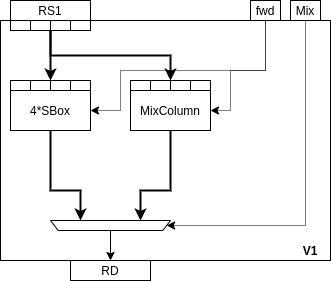
\includegraphics[width=\textwidth]{diagrams/ise-datapath-v1.png}
    \caption{\ISE{1}.}
    \label{fig:design:fu_block:v1}
\end{subfigure}
\begin{subfigure}[t]{0.40\textwidth}
    \centering
    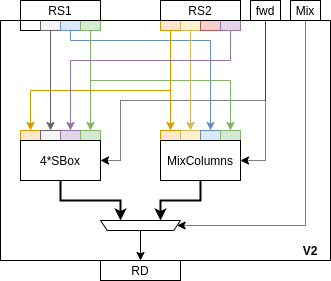
\includegraphics[width=\textwidth]{diagrams/ise-datapath-v2.png}
    \caption{\ISE{2}.}
    \label{fig:design:fu_block:v2}
\end{subfigure}

\begin{subfigure}[t]{0.40\textwidth}
    \centering
    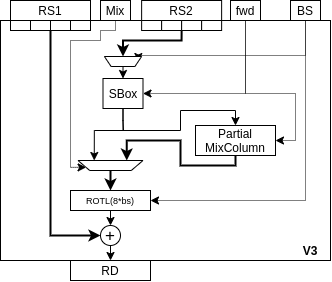
\includegraphics[width=\textwidth]{diagrams/ise-datapath-v3.png}
    \caption{\ISE{3}.}
    \label{fig:design:fu_block:v3}
\end{subfigure}
\begin{subfigure}[t]{0.40\textwidth}
    \centering
    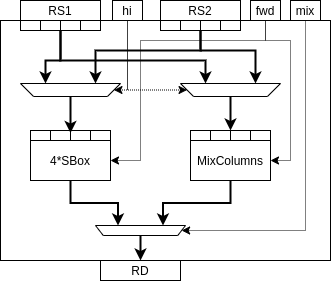
\includegraphics[width=\textwidth]{diagrams/ise-datapath-v5.png}
    \caption{\ISE{5}.}
    \label{fig:design:fu_block:v5}
\end{subfigure}
\label{fig:design:fu_block}
\caption{
A block diagram for each ISE variant, illustrating the associated AES functional unit.
}
\end{figure}

% -----------------------------------------------------------------------------

\REFSEC{sec:bg:aes_impl_ise}
outlined a range ISE designs, which constitute a large design space of
options that we {\em could} consider.  To narrow the design space into
those we {\em do} consider, we use the requirements as outlined below:

\begin{requirement}
The ISE should align with the wider RISC-V ethos and design principles.
Foremost, this means it should 
1) favour simple building-block operations,
   and
2) permit a $3$-address instruction format
   (resp. $2$-read, $1$-write register file port constraint).
\end{requirement}

\begin{requirement}
The ISE should operate on 
the RISC-V general-purpose scalar register file 
(i.e., st. $w \in \SET{32,64}$),
vs. 
any                        vector register file
(e.g., $w \ge 128$).
Note that this requirements excludes most standard ISEs outlined in 
\REFSEC{sec:bg:aes_impl_ise}.
\end{requirement}

\begin{requirement}
The ISE should introduce no
special-purpose       architectural state, 
nor rely on
special-purpose micro-architectural state
(e.g., caches or scratch-pad memory).
\end{requirement}

\begin{requirement}
The ISE should afford data-oblivious execution of AES, and thus prevent 
(digital) side-channel attacks based on execution time 
(e.g., stemming from accesses to the S-box).
\end{requirement}

% TODO: should we factor in memory footprint (and if so, how)

\begin{requirement}
The ISE must be efficient, in terms of improvement in latency per unit
unit of hardware required: this balances the value in both metrics, vs.
exclusively favouring one or the other.
\end{requirement}

\noindent
Overall, the requirements combine to intentionally target the ISE at 
 low(er)-end,
resource-constrained (e.g., embedded) platforms.  
We view such a focus as reasonable, because existing work on adding
cryptographic support to the
standard V 
(or vector) 
extension~\cite[Section 21]{RV:ISA:I:19}
already caters for
high(er)-end
alternatives.

We arrive at $5$ ISE varients, which are outlined in the following;
in each case, a dedicate \APPX contains additional technical detail, e.g.,
a complete list of instructions and their semantics, and examples of their
use when implementing AES.

% =============================================================================
